\documentclass[a4paper]{jsarticle}
\usepackage[dvipdfmx, hiresbb]{graphicx}
\usepackage[]{../math_note}
\usepackage[dvipdfmx, colorlinks=true]{hyperref}
\usepackage{pxjahyper}
\usepackage[]{enumitem}
\usepackage{listings, color}
\usepackage[all]{xy}

\usepackage{chngcntr}
\makeatletter
    \newcounter{c@question}
    \counterwithin{c@question}{section}
    \newenvironment{question}[0]%
    {\stepcounter{c@question}\begin{itembox}[l]{問\arabic{section}.\arabic{c@question}}}%
    {\end{itembox}}%
    \newenvironment{question*}[0]%
    {\stepcounter{c@question}\begin{itembox}[l]{問}}% 
    {\end{itembox}}%
\makeatother

\definecolor{dkgreen}{rgb}{0,0.6,0}
\definecolor{gray}{rgb}{0.5,0.5,0.5}
\definecolor{mauve}{rgb}{0.58,0,0.82}

\makeatletter
    \newcounter{c@problem}
    \counterwithin*{c@problem}{section}
    \newenvironment{problem}[0]%
    {\stepcounter{c@problem}\begin{itembox}[l]{問題\arabic{section}.\arabic{c@problem}}}%
    {\end{itembox}}%
    \newenvironment{problem*}[0]%
    {\stepcounter{c@problem}\begin{itembox}[l]{問題}}% 
    {\end{itembox}}%
\makeatother

\lstset{frame=tb,
  language=Python,
  aboveskip=3mm,
  belowskip=3mm,
  showstringspaces=false,
  columns=flexible,
  basicstyle={\small\ttfamily},
  numbers=none,
  numberstyle=\tiny\color{gray},
  keywordstyle=\color{blue},
  commentstyle=\color{dkgreen},
  stringstyle=\color{mauve},
  breaklines=true,
  breakatwhitespace=true,
  tabsize=3
}

\newcommand{\Sch}{\mathbf{Sch}}
\newcommand{\Set}{\mathbf{Set}}
\newcommand{\Ring}{\mathbf{Ring}}
\newcommand{\Alg}{\mathbf{Alg}}
\newcommand{\Cat}{\mathbf{Cat}}
\newcommand{\Open}{\mathrm{Open}}
\newcommand{\OpenSubSch}{\mathbf{OpenSubSch}}
\newcommand{\GrpSch}{\mathbf{GrpSch}}

\newcommand{\famF}{\mathcal{F}}
\newcommand{\famG}{\mathcal{G}}
\newcommand{\famU}{\mathcal{U}}

\newcommand{\spM}{\mathcal{U}}
\newcommand{\modM}{\mathcal{M}}

\newcommand{\ftor}[1]{\underline{#1}}
\newcommand{\ftorM}{\mathcal{M}}
\newcommand{\ftorGL}{\mathcal{GL}}

\newcommand{\mfor}{\text{for }}
\newcommand{\acton}{\curvearrowright}

\newcommand{\mat}[1]{\begin{bmatrix}#1\end{bmatrix}}

\begin{document}
\title{ゼミノート \#1 \\ Fine/Coarse Moduli Spaceの非存在}
\author{七条彰紀}
\maketitle

\begin{question}
    Fine/Coarse moduli spaceとは何か?
\end{question}
moduli spaceは``moduli functor"の情報を
可能な限り精密に写したschemeのことである.
その理解のためにはまず``functor of points"の概念が必要である.
以下,私が過去に書いたノート``Group Scheme"を引用・加筆する.

\section{Functor of Points}
    圏論で言う``generalized point"の概念を,
    名前を変えて用いる.

    \begin{Def}
    \enumfix
    \begin{enumerate}[label=(\roman*),leftmargin=*]
    \item 
    $X, T \in \Sch/S$に対し,
    $\ftor{X}(T)=\Hom_{\Sch/S}(T,X)$を\textbf{$X$の$T$-valued points}と呼ぶ.
    $T=\Spec R$と書けるときは$\ftor{X}(T)$を$\ftor{X}(R)$と書く.
    したがって$\ftor{X}$は$\Sch/S$からのcovariant functorと見ることも,
    $k$-algebraの圏からのcontravariant functorと見ることも出来る.
    この関手$\ftor{X}$はfunctor of pointsと呼ばれる.

    \item
    体$k$上のscheme :: $X$ ($S=\Spec k, X \in \Sch/S$)と
    field extension :: $k \subseteq K$について,
    $\ftor{X}(K)$を$X$の\textbf{$K$-rational points}と呼ぶ.

    \item
    morphism :: $h: X \to Y$について
    自然変換$\ftor{h}: \ftor{X} \to \ftor{Y}$は
    $\phi \mapsto h \circ \phi$のように射を写す.
    \end{enumerate}
    \end{Def}

    \begin{Remark}
        $\Sch$はlocally small categoryである.
        すなわち,任意の$X, T \in \Sch$について$\ftor{X}(T)$は集合である.
        これを確かめるために,
        $X, Y \in \Sch$を任意にとり,
        $\Hom(X,Y)$の濃度がある濃度で抑えられることを見よう.
        射$X \to Y$の作られ方に沿って考える.
        \begin{enumerate}[label=(\arabic*), leftmargin=*]
        \item
            base spaceの間の写像$f: \basesp X \to \basesp Y$をとる.
            このような写像全体の濃度は高々$|\basesp Y|^{|\basesp X|}$.
        \item
            $|Y|$の開集合$U$をとる.
            開集合全体の濃度は高々$2^{|\basesp Y|}$.
        \item
            写像$f^{\#}_U: \shO_Y(U) \to (f_* \shO_X)(U)$を定める.
            このような写像全体の濃度は高々$|(f_* \shO_X)(U)|^{|\shO_Y(U)|}$.
        \end{enumerate}
        したがって$\Hom(X,Y)$の濃度は高々
        \[|\basesp Y|^{|\basesp X|} \times \prod_{U \in 2^{\basesp Y}} |(f_* \shO_X)(U)|^{|\shO_Y(U)|} \]
        となる.
        濃度の上限が存在する(すなわち,ある集合への単射を持つ)から,
        $\Hom(X,Y)$は集合である.
%        presheaf on $Y$の圏は
%        $Y$の開集合が成す圏(small)から
%        集合の圏(locally small)の圏への
%        関手圏である.
%        これがlocally smallであることを示しても良いと思う.
    \end{Remark}

    \begin{Remark}
        上の注意から,Yoneda Lemmaが成立する.
        したがって自然変換$\ftor{G} \to \ftor{H}$と
        射$G \to H$が一対一対応する.
        このため,
        schemeの間の射についての議論と
        functor of pointsの間の射の議論は
        (ある程度)互いに翻訳することが出来る.
    \end{Remark}

    \begin{Remark}\label{remark:closedpoint}
        $K$-rational pointについては,
        $\ftor{X}(K)=\{ x \in X \mid k(x) \subseteq K \}$とおく定義もある.
        ここで$k(x)$は$x$でのresidue fieldである.
        しかし\cite{HarAG} Chapter.2 Ex2.7から分かる通り,
        この二つの定義は翻訳が出来る.
        すなわち,
        $k(x) \subseteq K$を満たす$x \in X$と,
        $\Spec k$-morpsihm :: $\Spec K \to X$は一対一に対応する.

        また$X$ :: finite type /$k$であるとき,
        closed point :: $x \in X$について,
        $k(x)$は$k$の有限次代数拡大体である.
        これはZariski's Lemmaの帰結である.
        したがって$\ftor{X}(\bar{k})$は$X$のclosed point全体に対応する.
        ただし$\bar{k}$は$k$の代数閉包である.
    \end{Remark}

    \begin{Example}
        $\R$上のaffine scheme $X=\Spec \R[x,y]/(x^2+y^2)$の
        $\R$-rational pointと$\C$-rational pointを考えよう.

        $\Spec \R \to X$の射は環準同型 $\R[x,y]/(x^2+y^2) \to \R$と一対一に対応する.
        しかし直ちに分かる通り,
        このような環準同型は
        \[ (\bar{x}, \bar{y}) \mapsto (0, 0) \]
        で定まるものしか存在し得ない.
        ここで$\bar{x}=x \bmod (x^2+y^2), \bar{y}=y \bmod (x^2+y^2)$と置いた.
        よって$\ftor{X}(\R)$は1元集合.
        また,この環準同型が誘導する$\Spec R \to X$の射は
        1点空間$\Spec \R$を原点へ写す.

        一方,環準同型 $\R[x]/(x^2+1) \to \C$は
        \[ (\bar{x}, \bar{y}) \mapsto (a, \pm ia) \]
        (ここで$i=\sqrt{-1}, a \in \R$)で定まることが分かる.
        すなわち,$\zerosa(x^2+y^2) \subseteq \affine^2_{\C}$の点に対応して,
        $\R[x]/(x^2+1) \to \C$の環準同型が定まる.
        逆の対応も明らか.
        よって$\ftor{X}(\C)$の元は
        $\zerosa(x^2+y^2) \subseteq \affine^2_{\C}$の点に
        対応している.
    \end{Example}

    \begin{Example}
        体$k$上のaffine variety :: 
        $X \subseteq \affine^n_k$を
        多項式系 :: $F_1,\dots,F_n \in k[x_1,\dots,x_n]$で定まるものとする.
        すると$k$上の環$R$に対して,次の集合が考えられる.
        \[ V_R=\left\{ p=(r_1,\dots,r_n) \in R^{\oplus n} ~\middle|~ F_1(p)=\dots=F_n(p)=0 \right\}. \]
        この集合の元も$R$-value pointと呼ばれる.
        (\cite{Muk1}ではこちらのみを$R$-value pointと呼んでいる.
        実際,こちらのほうが字句``value point"の意味が分かりやすいだろう.)
        $V_R$の点が$\ftor{X}(R)$の元と一対一に対応することを見よう.

        $X$のaffine coordinate ringを
        $A=k[x_1,\dots,x_n]/(F_1,\dots,F_n)$とし,
        $\bar{x}_i=x_i \bmod (F_1,\dots,F_n) ~(i=1,\dots,n)$とおく.
        $\phi: A \to R$を考えてみると,
        これは次のようにして定まる.
        \[ (\bar{x}_1,\dots,\bar{x}_n) \mapsto (r_1,\dots,r_n) \in V_R. \]
        すなわち,$V_R$の点に対して$\Hom_{\Ring/k}(A,R)$の元が定まる.
        逆の対応は明らか.
        そして,$\Hom_{\Ring/k}(A,R)$が
        $\Hom_{\Sch/\Spec k}(\Spec R, X)=\ftor{X}(R)$と一対一対応することはよく知られている.
    \end{Example}

\section{Moduli Functor and Fine/Corse Moduli Space}
    $A$を代数幾何学的対象の集合とし,
    $\sim$を$A$の中の同値関係とする.
    ``naive moduli problem"は,
    $M$の点\footnote{ \cite{GIT}では,特に$M$のgeometric point.定義は後述. }と
    $A/\sim$の元(同値類)が一対一対応するような
    scheme :: $M$を見つけよ,という問題である.
    更に$A/\sim$の元が「連続的に変化」する様子も
    「エンコード」しているような$M$を見つけよ,
    という問題を``extended moduli problem"と呼ぶ
    (正確な定義は\cite{Hos} \S 2.2).
    ``extended moduli problem"を定式化するには,
    「連続的に変化」と「エンコード」を定式化しなくてはならない.
    前者の為に``family"が定義され,
    後者の為に``moduli functor"が定義される.
    すると「エンコード」は関手の表現であると理解できる.
        射のfibreとして実現される,
        scheme(例えばsmooth curve)のfamilyは
        deformation theoryの対象である.

    \subsection{Families}
    \begin{Def}
        $\mathcal{P}$を集合のクラス
        \footnote
        {
            集合$X$を変数とする
            述語$X \in \mathcal{C}$の意味を
            「$X$はある条件を満たす対象である」と定義した,
            と考えて良い.
            「属す」の意味は集合と同様に定める.
        }
        とする.
        集合$B$について,
        $B$の構造と整合的な構造を持った集合$\famF$と
        全射写像$\pi: \famF \to B$の組が
        $\mathcal{P}$の$B$上の\textbf{family}であるとは,
        各$b \in B$について集合$\pi^{-1}(b) \subseteq \famF$が
        $\mathcal{P}$に属すということ.
%        $B$はfamily $\pi: \mathcal{F} \to B$のbaseと呼ばれる.
    \end{Def}
    「$B$の構造と整合的な構造」というのは,
    例えば,
    $S$が位相空間であって
    写像$\famF \to S$を連続にするような位相が$\famF$に入っている,
    ということである.
    familyの構造は場合毎に明示されなくてはならない.

    用語``family"を厳密に定義しているものは全くと言っていいほど無いが,
    ここではRenzoのノート
    \footnote{ \url{http://www.math.colostate.edu/~renzo/teaching/Topics10/Notes.pdf} }
    の定義を参考にした.
%    ただし,Renzoのノートの定義は一般化されすぎている.
%    Renzoのノートでは$\mathcal{P}$を
%    ``Let $\mathcal{P}$ define a class of objects in some category $\mathcal{C}$."
%    としているが,
%    これでは写像$\mathcal{F} \to B$が定義できるか怪しい.
%    なので私のこのノートでは$\mathcal{P}$を集合のクラスに限定している.
    ``family"を上のように解釈して不整合が生じたことは,
    私の経験の中ではない.

    \begin{Remark}
        moduli theory以外で``family of $\mathcal{C}$"と言えば,
        単に$\mathcal{C}$の部分集合であろう.
        ``family parametrized by $S$"の様に言えば,
        $S$-indexed family (or set)のことを想像するであろう.
        しかし$S$-indexed family :: $\famF \subset \mathcal{C}$は
        $S \to \famF$という写像で定まるから,
        ここでの``family"とは写像の向きが逆である.
        
        上の定義を無心に読めば分かる通り,
        「$\mathcal{C}$のfamily :: $\famF$」と言った時には,
        $\mathcal{C}$に属すのは$\famF$の部分集合である.
        属すのは(一般に)$\famF$の元ではない.
        また$\famF$は$\mathcal{C}$の元の和集合とみなせる.
        (正確には$\mathcal{C}$の元を$S$に沿って並べたものである.)
    \end{Remark}

    \begin{Example}
        $X, B$ :: scheme,
        $f: X \to B$ :: morphism of schemesをとる.
        $X$は$f$によって$B$上のfamilyとなる.
        $B$の点における$f$のfiberがmoduli問題の対象である.
        我々が代数幾何学の一分野としてModuli問題を扱う場合,
        現れるfamilyはこのようなもののみである.
    \end{Example}

    \begin{Example}\label{example:grassmannian}
        $k$を体,$S$を適当なschemeとする.
        $\affine^2_k$の原点を通る直線の$S$上のfamilyとして,
        line bundle :: $\shL \subset \affine^2 \times_k S$を
        考えることが出来る.
        $\shL \to S$は射影写像で与えられる.
        同様に$\affine^n$の$r$次元線形空間の$S$上のfamilyは
        $r$次元vector bundle :: $\shE \subset \affine^n \times S$である.
    \end{Example}

    \begin{Example}
        $k$を適当な体とし,
        $\proj^1_k$の点$O_i~(i=1,2,3)$を順に$(0:1), (1:0), (1:1)$とする.
        この時,$PGL_2(k)$は
        次の全単射で$\proj^1_k$の自己同型写像の$(\proj^1_k)^{\oplus 3}$上のfamilyになる.
        \begin{defmap}
            \pi:& PGL_2(k)& \to& (\proj^1_k)^{\oplus 3} \\
            {}& \phi& \mapsto& (\phi^{-1}(O_i))_{i=1}^3.
        \end{defmap}
    \end{Example}

    \begin{Remark}
        familyにしばしば要請される性質として,
        特に``flat"がある.
        projective flat familyは,
        base schemeに適切な条件をつけると
        各fiber :: $X_t$のHilbert多項式が$t$に依らない,
        という特徴がある(\cite{HarAG} III, Thm9.9).
        詳細は\cite{HarAG} III, 9を参照せよ.
    \end{Remark}

    \subsection{Moduli Functor}
    以下の定義は\cite{HaMo}など,
    Moduli問題に関する殆どの入門書で述べられている.
    \begin{Def}
        \textbf{moduli functor}(またはfunctor of families)とは,
        各scheme :: $S$に対して,
        $\ftorM(S)$が代数幾何学的対象の$S$上のfamily達を
        familyの間の同値関係で割ったもの
        (``$\{ \text{families over }S \}/\sim_S$" in \cite{Hos})である
        ような $\ftorM : \Sch \to \Set$のことである.
        morphism :: $f : S \to T$は,
        $\ftorM$によってpullbackに写される.
        すなわち,$\phi: \famF \to T$は$\ftorM(f)$によって
        $\famF \times_T S \to S$に写される.
        \[\xymatrix{
                \famF \times_T S \ar[d]_-{\ftorM(f)(\phi)}\ar[r]& \famF \ar[d]^-{\phi}\\
            S \ar[r]_-{f}& T
        }\]
    \end{Def}
    moduli functorの定義はあえて曖昧に述べられている.
    これは「出来る限り多くのものをmoduli theoryの範疇に取り込みたい」
    という思いがあるからである(\cite{HaMo}).

    \subsection{Fine Moduli Space}
    \begin{Def}
        scheme :: $M$が
        moduli fuctor :: $\ftorM$に対するfine moduli spaceであるとは,
        $M$が$\ftorM$を表現する(represent)ということである.
        言い換えれば,
        関手$\ftor{M}=\Hom_{\Sch}(-, M)$が$\ftorM$と自然同型,ということである.
    \end{Def}

    \begin{Remark}
        moduli functor :: $\ftorM$のfine moduli space :: $M$が存在したとしよう.
        この時,任意の$X \in \Sch$について$\ftorM(X) \iso \ftor{M}(X)$.
        これは
        $X$上のfamilyが成す同値類が
        $M$の$X$-valued pointと一対一に対応していることを意味する.
        したがって,
        $\ftorM$が指定する代数幾何学的対象の集合の同値類を
        $M$が「パラメトライズ」していると考えられる.
    \end{Remark}

    \begin{Def}
        moduli fuctor :: $\ftorM$に対する
        fine moduli spaceを$M$であるとする.
        また$\Psi: \ftorM \to \ftor{M}$を自然同型とする.
        $u=\Psi_M^{-1}(\id[M]): \famU \to M$をuniversal familyと呼ぶ.
    \end{Def}

    universal familyの名前の由来は次の命題に拠る.
    \begin{Prop}\label{prop:univfamily}
        任意のfamily :: $\phi: \famF \to B \in \ftorM(B)$は,
        $\chi=\Psi(\phi): B \to M$とuniversal family :: $u: \famU \to M$の
        pullback (fiber product)として得られる.
    \end{Prop}
    \begin{proof}
        $\Psi: \ftorM \to \ftor{M}$は自然同型であるから,
        $\chi=\Psi(\phi): B \to M$から次の可換図式が得られる.
        \[\xymatrix@=30pt{
                \ftorM(B) \ar[d]_-{\Psi_B}& \ftorM(M) \ar[l]_-{\ftorM(\chi)}\ar[d]^-{\Psi_M}\\
                \ftor{M}(B) & \ar[l]^-{\ftor{M}(\chi)} \ftor{M}(M) \\
        }\]
        $u \in \ftorM(M)$を$\ftorM(\chi)$で写すと$\famU \times_M B \to B$になる.
        同じ$u$を$\ftor{M}(B)$まで写すと,$\Psi_M(u) \circ \chi=\chi$になる.
        これを$\Psi_B^{-1}$で写せば$\phi:\famF \to B$.
        上の図式は可換図式であったから,
        $\phi=\famU \times_M B \to B$.
    \end{proof}

    \begin{Example}[\cite{Hos}, Exercise 2.20]
        例\ref{example:grassmannian}で述べた
        $\affine^n$の$r$次元線形空間の$S$上のfamily
        (vector bundle over $S$)の集合を,
        vector bundleの同型で割った集合を$\ftorM(S)$とする.
        $f: T \to S$に対する$\ftorM(f)$は,
        vector bundleへのpost-compositionで自然に定まる.

        このmoduli functorはfine moduli spaceを持つことが知られている.
        これがGrassmannian varietyである.
    \end{Example}

    残念ながら,多くのmoduli functorに対してfine moduli spaceが存在し得ない.
    (このあたりの議論は\cite{HaMo} p.3や\cite{HarDef} p.150にある.
    この節の終わりでも理由と例を示す.)
    そのためMumfordは\cite{GIT}で

    \subsection{Coarse Moduli Space}
    \begin{Def}\label{def:coarse-moduli}
        moduli functor :: $\ftorM$に対して,
        以下を満たすscheme :: $M$を$\ftorM$のcoarse moduli spaceと呼ぶ.
        \begin{enumerate}[label=(\roman*), leftmargin=*]
            \item
                自然変換$\Psi: \ftorM \to \ftor{M}$が存在する.
            \item
                $\Psi$はfunctor of pointsへの自然変換の中で最も普遍的である:
                \[
                \xymatrix
                {
                    {} & \ar[ld]_-{{}^{\forall} \tau}\ftorM \ar[rd]^-{\Psi}& {} \\
                    {}^{\forall}\ftor{\tilde{M}} & {} & \ar@{-->}[ll]^-{{}^{\exists_1} \ftor{f}} \ftor{M}
                }
                \]
                この図式で$\tilde{M}$ :: scheme, $f: M \to \tilde{M}$.
            \item
                任意の代数閉体$k$について,
                $\Psi_{\Spec k}: \ftorM(k) \to \ftor{M}(k)$は全単射である.
        \end{enumerate}
    \end{Def}
    条件(ii)は
    ``$M$ is the best (possible) approximation of $\ftorM$"だとか,
    ``$M$ is corepresent of $\ftorM$"と表現される.

    \begin{Remark}
        条件(ii)において$f$の向きを反転させると,
        coarse moduli spaceの定義が無意義に成る.
        実際,$f$の向きを反転させた条件を考えると,
        $\Sch$のinitial object :: $\emptyset$が条件を満たす.
        普遍ならば一意なので,
        任意のmoduli functorに対するcoarse moduli spaceは空集合$\emptyset$しかなくなる.
        これは条件(iii)を満たさないので,
        coarse moduli spaceは一切存在しないことに成る.
    \end{Remark}

    \begin{Remark}
        代数閉体$k$について,
        $\ftor{M}(k)$の元は``geometric point"と呼ばれる(\cite{GIT}, p.1).
    \end{Remark}

    \begin{Example}
        楕円曲線の$j$-invariant.
        後に示すとおり,これはfineでないcoarse moduli spaceである.
        自然変換$\Psi$は$j$-invariant(楕円曲線についての関数)を用いて
        \[ \Psi_S(\famF \to S): S \to \affine^1; \qquad s \mapsto j(\famF_s) \]
        のように定義できる.
        条件(iii)は\cite{HarAG} IV, Thm4.1で示されている.
        以下,条件(ii)を示す.

        ここでは\cite{HarDef} Prop 26.3の証明を参照した.
        \cite{JTev}では違う方針の証明が述べられている.
        
        $B=\Spec k[\lambda, 1/\lambda, 1/(1-\lambda)]$とし,
        family :: $\phi: \famF \to B$を
        $\lambda$をパラメータとするfamily :: $y^2=x(x-1)(x-\lambda)$で定める.
        $j$-invariantは
        \[ j(\lambda)=\frac{(1-\lambda+\lambda^2)^3}{\lambda^2(1-\lambda)^2} \]
        で定める.
        また,$\lambda \in B$を以下の$6$元のいずれかへ写す$6$つの$B$の自己同型群$G$は,
        $B$に作用する位数$6$の群となる.
        \[ \lambda, 1-\lambda, 1/\lambda, 1/(1-\lambda), (\lambda-1)/\lambda, \lambda/(\lambda-1). \]

        今,scheme :: $M'$と自然変換$\Psi': \ftorM \to \ftor{M'}$が存在したとしよう.
        $\phi:\famF \to B$の$\Psi'$による像を$\chi': B \to M'$とする.

        $y^2=x(x-1)(x-\lambda)$と$y^2=x(x-1)(x-(1-\lambda))$は同型であることが知られている.
        他の$1/\lambda, 1/(1-\lambda), \dots$についても同様である.
        $\chi'$はfiberの同型類と$M'$の点を($B$の$6$点を経由して)一対一対応させる.
        なので,任意の$g \in G$について$\chi' \circ g=\chi'$すなわち,
        $\chi'$は$G$-invariant mapである.

        $G$-invariant mapは$B$の$G$によるcategorical quotientを介する二つの射に分解される.
        GIT quotientの理論により,
        \[ B \sslash G=\Spec (k[\lambda]^G) \]
        がcategorical quotient(特にgood quotient.\cite{Hos}参照.).
        そしてこれは$\affine^1_{j}=\Spec k[j]$に等しい(\cite{HarAG} IV, Thm4.1参照).
        なので$\chi': B \to M'$は$B \to \affine^1_{j} \to M'$に分解される.
        こうして$\psi: \affine^1_{j} \to M'$が得られた.

        この$\psi$によって以下の図式が可換であることを確かめる.
        (TODO)
    \end{Example}

    \subsection{Properties of Fine / Coarse Moduli Spaces}
    \begin{Prop}
        moduli functor :: $\ftorM$に対して
        coarse moduli spaceは同型を除いて一意である.
    \end{Prop}

    \begin{Prop}[\cite{HarDef}, Prop23.6]
        scheme :: $M$が
        moduli functor :: $\ftorM$に対する
        fine moduli spaceであるならば,
        $M$は$\ftorM$のcoarse moduli spaceでもある.
    \end{Prop}
    この二つをまとめると次の図式に成る.
    \[\xymatrix{
        \text{Fine moduli} \ar@{=>}[r]& \text{Coarse moduli} \ar@{=>}[r]& \text{Universality} \ar@{=>}[d]\\
        {} & {} & \text{Uniqueness}
    }\]

    \begin{Prop}
        $M$をmoduli functor $\ftor{M}$のcoarse moduli spaceとする.
        また$\Psi: \ftorM \to \ftor{M}$を自然変換とする.
        $M$がfine moduli spaceであることは次と同値.
        \begin{enumerate}
            \item $\Psi(u)=\id[M]$となるfamily :: $u: \famU \to M$が存在する.
            \item 任意のscheme :: $S$について$\Psi_S: \ftorM(S) \to \ftor{M}(S)$は単射.
        \end{enumerate}
    \end{Prop}
    \begin{proof}
        $M$がfine moduli spaceである(すなわち$\Psi$が自然同型である)ときに
        $2$条件が成り立つことは明らか.

        任意のscheme :: $S$について$\Psi_S$が同型(iso)であることを示す.
        今,$\ftorM(S), \ftor{M}$がどちらも集合であるから,
        $\Psi_S$は写像である.
        iso mapはsurj+inj mapと同値であるから,
        我々は$\Psi_S$ :: surjのみ示せば良い.
        しかしこのことは命題\ref{prop:univfamily}で証明されている.
    \end{proof}
    
    \begin{Prop}[\cite{HarDef}, Prop23.5]
        $S$ :: schemeのopen subschemeと包含写像が成す圏を
        $\OpenSubSch(S)$と書くことにする.
        これは$\Sch/S$のfull subcategoryである.

        moduli functor :: $\ftorM$が
        fine moduli spaceをもつならば,
        任意の$S$ :: schemeについて
        $\ftorM|_{\OpenSubSch(S)}$は$S$上のsheafである.
        言い換えれば,
        $\ftorM$はZariski topology上のsheafである.
    \end{Prop}
    \begin{proof}
        $M$ :: fine moduli scheme for $\ftorM$とし,
        $S$ :: schemeを固定する.
        $\shF:=\ftor{M}|_{\OpenSubSch(S)}$は
        開集合系からのcontravariant functorだから
        presheafであることは定義から従う.
        また$\shF$の元はschemeのmorphismである.
        このことからsheafの公理Identity AxiomとGluability Axiomを
        満たすことも簡単に分かる.
        (一応,\cite{HarAG} II, Thm3.3 Step3を参考に挙げる.)
    \end{proof}

    \begin{Remark}\label{remark:trivfamily}
        それぞれのfiberが互いに同型である
        (i.e. $\Forall{t,s \in S} \famF_t \iso \famF_s$)ような
        familyをfiberwise trivial family, 
        対象$X$(なめらかな曲線など)を用いて
        $X \times S \to S$の形に書けるfamilyをtrivial familyと呼ぶ.

        fine moduli spaceが存在するならば,
        fiberwise trivial familyはtrivial familyである
        (cf. \cite{HarDef} Remark 23.1.1).
        実際,任意のfiberが$X$と同型であるようなfamily :: $\famF \to S$
        から得られる$\Psi_S(\famF \to S): S \to M$は
        $X$に対応する点へのconstant mapになっている.
        $\Psi_S(X \times S \to S)$も明らかに同じconstant mapとなるから,
        $\Psi_S$ :: isomorphismより
        $X \times S \to S \sim \famF \to S$.
    \end{Remark}

\section{Non-existence of Fine/Coarse Moduli Space}
    \begin{question}
        Fine/Coarse Moduli Spaceはいつ存在するのか?
    \end{question}
    十分条件を示すのではなく,
    \footnote
    {
        十分条件については次の命題が有る:
        \url{ https://stacks.math.columbia.edu/tag/01JJ }.
        次のページでは,
        この命題を用いてGrassmannian functorが表現可能であることを示している:
        \url{ https://stacks.math.columbia.edu/tag/089R }.
    }.
    ここでは問を次のように限定する.
    \begin{question}
        Fine/Coarse Moduli Spaceはいつ存在しないのか?
    \end{question}

    Moduli問題の対象と一対一に対応するschemeが見つかったからと言って,
    それがfine moduli spaceであるとは言えない.
    問題と成るのは,familyの同型である.
    以下では特にautomorphismの存在とjump phenomenonが
    fine moduli spaceが存在するための障害と成ることを見る.

    注意 (\ref{remark:trivfamily})の内容
    を用いて証明する.

    \subsection{\texorpdfstring{$j$}{j}-invariant is not a fine moduli space.}
    一つ例を見よう.

    $S=\affine^1_k-\{0\}$とする.
    $S$上の楕円曲線のfamily :: $\famF$を次で定める.
    \[
        \famF=\zerosa(y^2-x^3-s) \subseteq \affine^2_k \times_k S
        \xrightarrow{\pr} S.
    \]
    $\Psi(\famF)$を$j$不変量を用いて$s \mapsto j(\shF_s)$で定める.
    $j$不変量がcoarse moduliであることは既に見た.
    計算すると分かる通り,$\Psi(\famF)$は定値写像である.
    したがって$\famF$のそれぞれのfiberは互いに同型である.
    一方,$\famF'=\zerosa(y^2-x^3-1) \times S$について
    同様に$\Psi(\famF')$を定めると,
    これも自明に定値写像である.
    しかし,$\famF \not \iso \famF'$であることが示せる.
    よって注意 (\ref{remark:trivfamily})から$j$不変量はfine moduliにならない.
    fine/coarse moduliの一意性から,
    楕円曲線はfine moduliを持たない.
    \begin{proof}[proof of $\famF \not \iso \famF'$]
        \cite{HarAG} I, Ex6.2を参考にする.
        我々が調べるのは次の二つの環である.
        それぞれ$\famF, \famF'$である.
        \[
            A=k[x,y, t,t^{-1}]/(y^2-x^3-t),
            \qquad
            B=k[x,y]/(y^2-x^3-1) \otimes_k k[t,t^{-1}],
        \]
        $A$はUFDであるが$B$はUFDでない(GCD domainでさえない),
        ということを示す.

        $A$は$k[x,y]_{y^2-x^3}$(1元での局所化)と同型である.
        $k[x,y]$はUFDであり,irreducible elementでの局所化でこれは保たれる.
        すなわち$A$はUFD.

        $B$がUFDでないことを示すために,
        $\bar{x}=x \bmod (y^2-x^3-1)$がnot primeだがirreducibleであることを示す.

        $\bar{x}$ :: not primeを示すために次の等式を考える.
        \[ \bar{x}^3=\bar{x} \cdot \bar{x} \cdot \bar{x}=(\bar{y}+1) \cdot (\bar{y}-1). \]
        $\bar{x}$ :: primeと仮定すると,
        $\bar{y}+1 \mor \bar{y}-1 \in (\bar{x})$となる.
        そこで例えば
        \[ \bar{y}+1=a \bar{x} \]
        なる$\bar{a} \in B$が存在するとしよう.
        すると$y+1-a x \in I$が得られる.
        これは楕円曲線$y^2=x^3+1$が$y+1-a x=0$という曲線に含まれていることを意味する.
        したがって$x=0$と楕円曲線の交点は,
        存在しても$(x,y)=(0,-1)$の一つのみ,ということになる.
        しかし実際は$(0,-1)$もこの楕円曲線に属すので矛盾.

        $\bar{x}$ :: irreducibleを示すために$\sigma$と$N$を準備する.
        $\sigma: k[x,y] \to k[x,y]$を$y \mapsto -y$で他の元は変化させないものとする.
        すると$\sigma(I) \subseteq I$なので$\sigma: B \to B$が誘導される.
        さらに$N(a)=a \cdot \sigma(a)$で$N: B \to k[\bar{x}]$を定める.
        $N$は積について準同型であることに注意せよ.

        $\bar{x}$がirreducibleでないならば,
        $\bar{x}=fg \bmod I$なる$f,g \in k[x,y]$が存在する.
        $f \bmod I, g \bmod I$はどちらも単元でない.
        両辺を$N$で写すと次のように成る.
        \[ (x^2-N(f)N(g)) \bmod I=0. \]

        したがって$x^2-N(f)N(g)=a(y^2-x^3-1)$なる$a \in k[x,y]$が存在する.
        左辺は$k[x]$に属すから,$y$の次数を考えると$a=0$が示される.
        また$N(f), N(g)$の次数は$2$以上であるから,
        $N(f), N(g)$のいずれかは$k^{\times}$の元である.
        しかし$N(f)=f \cdot \sigma(f)$ (resp. $N(g)$)が単元ならば$f$ (resp. $g$)も単元であり,
        $f,g$についての仮定に反する.
        よって$\bar{x}$ :: irreducible.
    \end{proof}

    したがってmoduli functorは必ずしもfine moduli spaceを持たない.

    \subsection{Automorphism is an obstruction to the existence of fine moduli space.}
    Moduli問題の対象が非自明な自己同型写像をもつなら,
    多くの場合でfine moduli spaceが存在し得ない.

    例を二つ考える.
    最初の例は構成の仕方がschemeaticでないが,
    直観的である.
    \begin{Example}
        $k$ :: fieldとし,
        $\affine^2_k$の原点を通る直線を,\kenten{同型を無視して}分類する.
        直線は全て同型であるから,これは一つしか無い.
        したがってこの問題に対するfine moduli spaceが存在すれば,
        それは一点空間である.
        したがって任意のscheme :: $B$について,
        $B$上のfamilyは全てtrivial familyと同型である.
        
        $L$を$\affine^2$の原点を通る直線とし,
        その非自明な自己同型$\sigma: L \to L$をとる.
        $[0,1]$上のtrivial fiber :: $[0,1] \times L$を,
        次の同値関係で割って商空間を作る.
        \[ (t, Q) \sim (s, Q) \iff |t-s|=1 \land P=\sigma(Q) \mwhere s,t \in [0,1], P,Q \in L. \]
        例えば$\sigma$を$(x,y) \mapsto (-x,-y)$と置くと,
        これは丁度メビウスの帯である.
        そしてこれは$S^1$上のfamilyとなっている.

        今$S^1$上のfamilyとして,
        $\sigma$を使って構成したもの(メビウスの帯)とtrivial family (斜めになった円筒)がある.
        これらは明らかに同型ではない.
    \end{Example}

    \begin{Example}
        scheme :: $B$とfamily over $B$ :: $X$を次のように定める.
        \[
            B=\Spec \C[\lambda, (\lambda(1-\lambda))^{-1}] =\affine_{\C}^1-\{0,1\},
            \qquad
            X=\Proj \frac{\C[x,y,z, \lambda, (\lambda(1-\lambda))^{-1}]}{(y^2z-x(x-z)(x-\lambda z))}
            \subset \proj^2_{\C} \times_{\C} B.
        \]
        任意の$\C$上の楕円曲線と同型なものがfamily :: $\pr: X \to B$に含まれている.
        そして$j$-invariant :: $A^1_{[j]}$は$B$の次の群$G$による商として得られる
        (このことは\cite{HarDef} Prop 26.3の証明で示されている).
        \[ G=\left\{ \lambda \mapsto \frac{a-b}{c-b} ~\middle|~ \{a,b,c\}=\{0,1,\lambda\} \right\}. \]
        したがって$\C$上の楕円曲線のuniversal familyは,
        ``quotient of family" $X/G \to B/G=\affine^1_{[j]}$として得られるはずである.
        同型なfiberはひとつのfiberにまとめてしまえば,
        同型類の代表をひとつづつfiberにもつfamilyが作れるであろう,
        というわけである.
        \begin{center}
            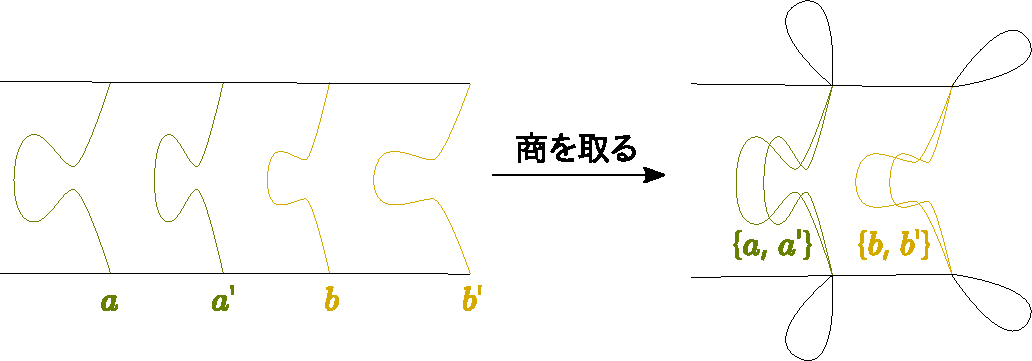
\includegraphics[width=9cm,pagebox=cropbox]{./images/quotient_of_family.pdf}
        \end{center}

        問題は$X/G$である.
        $X/G$に言及するには$G$の$X$への作用を定める必要が有るが,
        楕円曲線には非自明な自己同型があるため,
        奇妙な族を作ることが出来る.
        これは以降の段落でもう少し具体的に述べる.
        もし楕円曲線の族のfine moduli spaceが存在するならば,
        fine moduli spaceも,universal familyも,同型を除いて一意である.
        なので,$X/G \to B/G$が唯一の候補である.
        しかし$X/G \to B/G$は楕円曲線の族ではない.
        したがって楕円曲線のuniversal familyは存在せず,
        fine moduli spaceも存在しない.

        ここでは$B/G$でなく,
        $G$の元$\sigma$で生成される$G$の部分群$G'=\{\id, \sigma\}$による商$B/G'$を考える.
        \[ G \ni \sigma: \lambda \mapsto \frac{\lambda-1}{0-1}=1-\lambda. \]
        $\sigma$はinvolution(i.e. $\sigma \circ \sigma=\id$)である.
        対して$X$の自己同型を次のように取る.
        \[ \tau: (x,y,z, \lambda) \mapsto (x,-y,z,1-\lambda). \]
        こちらも$\sigma$同様involutionである.
        そして$\tau$は$\sigma: \affine^1 \to \affine^1$の持ち上げである.
        すなわち,次の図式は可換である.
        \[\xymatrix{
                X \ar[r]^-{\tau}\ar[d]_-{\phi}& X \ar[d]^-{\phi}\\
                \affine^1 \ar[r]_-{\sigma}& \affine^1
        }\]
%        $\tau$は同型なので,これはpullback図式でもある.
%        なのでpullback lemmaから,
%        以下の図式の一番外側の四角形もpullback図式である.
%        \[\xymatrix{
%                X \ar[r]^-{\tau}\ar[d]_-{\pr}& X \ar[d]_-{\pr} \ar[r]& U \ar[d]^-{\mathbf{1}}\\
%                \affine^1 \ar[r]_-{\sigma}\ar@/_15pt/[rr]_-{j}& \affine^1 \ar[r]_-{j}& \affine^1_{[j]} \\
%        }\]
        
        今,$H'=\{\id, \tau\}$は明らかに$X$に作用する.
        そして上の図式が可換であることから,family :: $\phi: X/H' \to B/G'$が得られる.
        そこでこのfamilyを考えてみると,
        $\sigma$の不動点$\lambda=1/2$における$\phi$のfiber$\phi^{-1}(1/2)$は,
        $X_{1/2}$の$\tau_{1/2}:(x,y,z) \mapsto (x,-y,z)$による商となっている.
        この商は,Riemann-Hurwitzの公式によると,genusが$0$となっている
        \footnote
        {
            楕円曲線はgenusが$1$で,$0,1,\lambda, \infty$の$4$点で分岐しており,
            この$4$点それぞれの分岐指数は$2$である.
            $\phi^{-1}(1/2)$は商写像$X_{1/2} \to X/\tau_{1/2}$による2重被覆だから,
            $\phi^{-1}(1/2)$のgenusを$h$とすると,
            $2-2 \cdot 1=2h-4 \cdot (2-1)$.
            故に$h=0$.
        }.
        しかし楕円曲線の種数は$1$でないから,
        $\phi$は楕円曲線の族ではない.
        同様にして$X/G \to B/G$も楕円曲線ではないように作用$G \acton X$を作れる.
    \end{Example}

    より抽象的な設定で証明しよう.
    これもfiberwise trivial but non-trivial familyを構成すれば良い.
    ここでは\cite{IntroFam} \S4.8.2と
    M.Hoeveのノート``An Introduction to Moduli Spaces of Curves"
    Example 3.2を参照した.
    他,
    D.Eisenbud and J.Harris ``Schemes:The Language of Modern Algebric Geometry"
    IV.B\ viiにも同様のことが記述されているのを発見した.
    \begin{Example}
        $X$をscheme over $\Z$とし,
        これがnon-trivial automorphism :: $\sigma: X \to X$を持つとする.

        order of $\sigma$を$n$とする.
        すなわち,$n$を$\sigma^n=\id$となる最小のものとする.
        $n$は$2$以上の整数または無限大である.
        $\sigma$で生成される群を$G_{\sigma}$とする.
        これはcyclic group of order $n$.

        base of familyとなるscheme :: $B$と
        $B$のnon-trivial isomorphism :: $\tau: B \to B$を定める.
        これは$n$の値で場合分けすれば具体的に与えることが出来る.
        \begin{description}
            \item[$n=2$: ] 
                $B=\proj^1-\{(\pm 1:1)\}$とし,
                $\tau$を座標の交換$(x:y) \mapsto (y:x)$とする.
            
            \item[$2<n<\infty$: ]
                $B=\proj_{\C}^1-\{(\pm i:1)\}$とし,
                $\tau$を$2 \pi/n$回転
                (アフィン平面の回転から誘導されるもの)とする.

            \item[$n=\infty$: ]
                $B=\affine_{\C}^1$とし,
                $\tau$を$z \mapsto z+2 \pi i$とする.
        \end{description}
        いずれの場合でも$\tau$で生成される群$G_{\tau}$は
        cyclic group of order $n$であり,
        $\psi: \sigma \mapsto \tau$によって
        $G_{\sigma}$と同型である.
        さらに$\tau$は固定点をもたず,
        $B$はsmooth irreducible scheme over $\C$となっている.

        $G_{\sigma}$の$X \times B$への作用を次で定める
        \footnote
        {
            \cite{IntroFam} \S4.8.2ではこの辺りに大きな間違いがある.
        }.
        \begin{defmap}
            \alpha:& G_{\sigma} \times (X \times_{\Z} B)& \to& X \times_{\Z} B \\
            {}& (g, (x, b))& \mapsto& (g(x), \psi(g)(b))
        \end{defmap}
        $B$にも$G_{\sigma}$の自明な作用を与えると,
        $\phi: (X \times B)/G_{\sigma} \to B/G_{\sigma}$が得られる.

        この時,
        $\phi: (X \times B)/G_{\sigma} \to B/G_{\sigma}$は
        fiberwise trivial but non-trivial familyである.
        \begin{proof}
            (TODO)
        \end{proof}
    \end{Example}

    \subsection{Jump Phenomenon.}
    coarse moduli spaceさえ持ち得ないmoduli functorもある.

    \begin{Prop}[\cite{Hos} Lemma2.27, \cite{HarDef}]
        moduli functor :: $\ftorM$を考える.
        さらに$\ftorM$とは無関係に
        algebraically closed field :: $k$をとる.
        family :: $\famF \to \affine_k^1 \in \ftorM(\affine_k^1)$が
        以下の条件を満たすと仮定する.
        すると$\ftorM$のcoarse moduli spaceは
        finite type over $k$\kenten{ではない}.
        この条件とはすなわち:
        \[
            \famF_{s} \sim \famF_{t}
            \ \mand\ 
            \famF_{0} \not \sim \famF_{s} \quad (\mfor s,t \in \affine^1-\{0\}).
        \]
        
        特にthe best approximation of $\ftorM$ 
        (定義\ref{def:coarse-moduli}直後)が
        代数閉体上finite typeなschemeであった場合,
        $\ftorM$はcoarse moduli spaceを持たない.
    \end{Prop}
    命題の条件を満たすfamilyを,
    jump phenomenonが起きているfamilyと呼ぶ.
    \begin{proof}
        代数閉体$k$上finite typeなscheme :: $M$をとり,
        自然変換$\Psi: \ftorM \to \ftor{M}$が存在したとしよう.
        主張にあるfamily :: $\famF \to \affine^1$を$\Psi$で写したものを
        $f: \affine^1 \to M$としよう.

        $\affine^1$のclosed pointsは$M$のclosed pointに写る
        \footnote
        {
            finite type over an algebraically closed fieldという条件は,
            このことを示すために付いている.
            実際のところは``$M$ :: Jacobson and $f$ :: locally finite type"
            という条件が必要十分である.
            詳細は\url{ https://stacks.math.columbia.edu/tag/01TB }を参照して欲しい.
            この必要十分条件が成立する典型例が今回の$M,f$の条件である.
        }.
        $k$ :: algebraically closed fieldかつ
        $\affine_k^1, M$共にfinite type over $k$であるから,
        closed pointsを考えることは$\Spec k$からの射を考えることに等しい.
        今,functor of pointsの間のnatural transformation :: 
        \[ \ftor{f}(k): \ftor{\affine^1}(k) \to \ftor{M}(k) \]
        による$\ftor{\affine^1}(k) \ni s: \Spec k \to \affine^1$の像は,
        $\ftor{f}(s) \in \ftor{M}(k)$である.
        このことをclosed pointsの言葉に書きなおせば:
        closed point :: $s(\Spec k) \in \affine^1$の像は$M$のclosed point.
        
        $f$がcoarse moduli spaceならば,
        $\Psi_k: \ftorM(k) \to \ftor{M}(k)$は全単射である.
        $s \in \affine^1$に対応する$\Spec k \to \affine^1$を$\bar{s}$と書くことにすると,
        \[ \ftor{f}(\bar{s})=f \circ \bar{s}=\Psi_k(\famF_s): \Spec k \to M. \]
        $s \neq 0$ならば,
        $\famF_s \not \sim \famF_0$なので$\Psi_k(\famF_s) \neq \Psi_k(\famF_0)$.
        これは$\Spec k$は1点空間だから,これは次と同値.
        \[ (f \circ \bar{s})(\Spec k)=f(s) \neq f(0)=(f \circ \bar{0})(\Spec k). \]
        $s, t \neq 0$ならば$\famF_s \sim \famF_t$であるから,
        合わせて$f^{-1}(f(\{0\}))=\affine^1-\{0\}$となる.
        これはclosed subsetではない.
        しかし$f(\{0\}) \subset M$はclosed setであり,
        かつ$f$は連続であるから,
        これは有り得ない.
    \end{proof}
    \begin{Remark}
        命題中の$\affine^1$と$0 \in \affine^1$は,
        より一般に
        connected scheme of finite type over an algebraically closed fieldと
        closed pointに置き換えられる.
        connectedはclosed pointの補集合がclosedにならないために必要である.
        $M$の条件「finite type over $k$ではない」についても,
        脚注の通り一般化出来る.
    \end{Remark}

    \begin{Example}[\cite{HaMo} Exercise (1.7)]
        moduli functor :: $\ftorM$を,
        ``flat families of reduced plane curves of degree 2 over $\C$, up to isomorphism"
        のmoduli functorとして定める.
        ただし,ここでは$\affine_{\C}^2$の曲線を考える.
        $\ftorM(\C)$の元,すなわち``reduced plane curves of degree 2"の同型類は
        2つしかないことに注意する.

        以下,the best approximation of $\ftorM$は$\Spec \C$であることを示す.
        $t$-line :: $\affine_{\C}^1$上のfamily :: $xy=t$でjump phenomenonが起きるため,
        $\ftorM$はcoarse moduli spaceを持たない.

        \begin{proof}
        \paragraph{There exists natural transformations $\ftorM \to \ftor{\C}$.}
        $\ftorM(B) \ni \phi: \famF \to B$に対し,
        $\Psi(\phi) \in \ftor{\C}(B)$を次のように定める.
        $b \in B$について$\famF_b \subseteq \affine^2_{\C}$であることに注意せよ.
        \[ B \ni b \mapsto \famF_b \xrightarrow{\pr} \affine^1_{\C} \xrightarrow{\pr} \Spec \C \]
        これは自然変換である.
        よって$\ftorM \to \ftor{M}$の自然変換が存在する.

        \paragraph{The best approximation of $\ftorM$ is $\Spec \C$.}
        scheme :: $M'$と自然変換
        $\Psi': \ftorM \to \ftor{M'}$をとって固定する.
        $\Psi$は引き続き自然変換$\ftorM \to \ftor{\C}$とする.
        $\phi: \famF \to B$ :: flat family of smooth conicとする.
        このfamilyはfiberwise trivial familyだから,
        $\Psi'_B(\phi): B \to X$は定値写像である.
        その値を$x \in X$とすると,
        包含写像$k(x) \inclmap \C$から
        射$\pi: \Spec \C \to X$が定まる(\cite{HarAG} II, Ex2.7).
        これは$\pi(\Spec \C)=\{ x \}$を満たす.
        この射に依って$\Psi'(\phi)=\pi \circ \Psi(\phi)$となることは明らか
        (TODO: どうすれば$k(x) \inclmap \C$の存在が保証できる?).
        \end{proof}
    \end{Example}

%    あるいはmoduli fuctorが``unbounded"であるときに起きる.
%    このノートでは深追いしない.
%    詳しくは\cite{Hos} \S 2.4を参照せよ.

\section{Dealing with Non-existence of Fine/Coarse Moduli Space.}
    fine moduli spaceが存在するための障害を
    回避する方法は幾つかある.
    
    以下,moduli問題の対象をobjectと呼ぶ.

    \subsection{Sub-Moduli Functor of ``Objects Without Non-Trivial Automorphism".}
    考えているmoduli問題を修正し,
    対象を自明な自己同型しか持たないものに限定する.
    すると多くの場合でfine moduliが存在しうる.
    しかし,この修正されたmoduli問題が解けても,
    元のmoduli問題に関する情報が殆ど出てこないことが多い.

    \subsection{Rigidifying of Moduli Problem.}
    これは,追加の情報を考慮に入れることで,
    objectsを予め大雑把に分類しておく,
    ということである.
    追加の情報としては以下のようなものが考えられる.
    \begin{enumerate}
        \item fixed sub-objects.
        \item level structure.
        \item ordered sets of (higher-order) Weierstrass points.
    \end{enumerate}

    \subsubsection{ Fixed Sub-object }
    fixed sub-objectsは,
    例えば幾つかの固定された点を通る曲線のmoduli問題を考えるということである.
    この場合,十分に固定点の個数を大きくすれば,
    non-trivial automorphismが存在しなくなる.
    この修正によって得られるmoduli spaceが
    どれだけ元の問題のmoduliを反映しているか,
    というのは不透明である.
    しかしこの修正はしばしば自然に現れる.

    \subsubsection{ Level Structure }
    level structureはirreducibility of $\modM_g$を証明する際に導入された.
    level structureを考慮してmoduli問題を修正すると,
    元の問題のmoduli spaceのfinite coverが得られる.
    level $n$, genus $g$のcurveのmoduli spaceを$\spM_g^{(n)}$と書く.

    level structureは様々な定義が存在する.
    abelian schemeのlevel structureの定義は
    \cite{GIT} p.129, Definition 7.1にある.
    これはabelian schemeのmoduli spaceを研究するために用いられている.
    特にelliptic curve over $\C$のWeil paring, level structureについては,
    \cite{DiaShur}に詳しい記述がある.
    F.Volochによるcourse noteにも整理された記述がある.
    \footnote{\url{ https://www.ma.utexas.edu/users/voloch/390-10.html }}
    また,symplectic level structureは\cite{CFMSC}で整理されている.
    Teichm\"uller structure of level $G$ ($G$は有限群)は
    \cite{IrrOfMg}で導入されている.

    ここではHesse cubic formを用いて,
    代数閉体$k$($\fchar k \neq 3$)上の楕円曲線のlevel $3$-structureと,
    level $3$-structureを持つ楕円曲線のmoduli spaceを解説する.
    参考文献は二つ:
    \url{https://arxiv.org/abs/math/0611590}, 
    \url{http://www.math.chalmers.se/~ulfp/Teaching/AG.html}.

    $k$を$\Z[1/3, \xi]/(\xi^2+\xi+1)$を含む体,
    すなわち,標数が$3$でなく$1$の原始$3$乗根を持つ体とする.
    $k$上の楕円曲線$E$を予め埋め込んで射影平面上のものと考える.
    $E$のlevel $3$-structureとは,
    $(\Z/3\Z)^2$とgroup of $3$-torsion points in $E$ :: 
    \[ E[3]=\{ P \in E \mid 3P=O. \} \]
    の間の同型$\alpha: (\Z/3\Z)^2 \to E[3]$のことである.
    この同型は$\alpha(0, 1)$と$\alpha(1, 0)$の点を与えれば定まることに注意する.

    この同型$\alpha$が存在することは,以下のように分かる.
    具体的な考察により,$E[3]$の元は,その$1$点のみで$E$と交わる点,
    すなわち変曲点であることが分かる.
    これは$E$が$3$次曲線であることから,これは$9$点存在する.
    すなわち$E[3]$は位数$9$のアーベル群.
    アーベル群の構造定理と,$E[3]$の任意の元の位数が高々$3$であることから,
    $E[3] \iso (\Z/3\Z)^2$が分かる.

    我々がこれから主張することは,
    \[ B=\affine^1-\{ 1, \xi, \xi^2 \} \]
    がlevel $3$-structureを持つ$k$上の楕円曲線のfine moduli spaceであることである.
    まずlevel $3$-structureを持つ$k$上の楕円曲線のfamilyを考える.
    $S$を$k$上のschemeとして,楕円曲線とその$2$つの$3$-torsion pointのfamilyを取る.
    
    $k$上の楕円曲線$E$とlevel $3$-structure :: $\alpha: (\Z/3\Z)^2 \to E[3]$をとる.
    埋め込み$i: E \to \proj_k^2$の像と$i \circ \alpha$をとれば,
    最初から$E$は$\proj^2$内の楕円曲線と考えられる.
    $E$を以下のような写像で写す.
    \[
        \alpha(0,0) \mapsto (0:1:-1), \quad
        \alpha(1,0) \mapsto (0:1:-\xi), \quad
        \alpha(0,1) \mapsto (-1:0:1), \quad
        \alpha(1,1) \mapsto (-\xi:0:1).
    \]
    このような$\proj^2$の自己同型はただひとつ存在する.
    そしてこれは$E[3]$の群構造を維持し,
    像は以下の$9$点を通る.
    \[ K=\{ (0:1:-\beta) : (-\beta : 0 : 1), (1 : -\beta : 0) \mid \mwhere \beta^3=1 \}. \]
    $\proj^2$の種数$1$の曲線は$3$次曲線である.
    そして以上の$9$点を通る非特異曲線は,以下の形の多項式で定義される.
    \[ x^3+y^3+z^3-3 \mu xyz=0 \]
    こうして$(E, \alpha)$から$\mu \in B$への写像が定まる.
    この楕円曲線の$3$-torsion pointsは上の$9$点である.
    
    逆に,Hesse pencil
    $H_{\mu}: x^3+y^3+z^3-3 \mu xyz=0$をとる.
    これのlevel $3$-structureは
    \[
        \alpha(0,0) \mapsto (0:1:-1), \quad
        \alpha(1,0) \mapsto (0:1:-\xi), \quad
        \alpha(0,1) \mapsto (-1:0:1).
    \]
    で定まる.

    level $3$-structureのとり方には$SL(2, \Z/3\Z)$の自由度がある.
    より具体的には$M \in SL(2, \Z/3\Z)$について,
    以下のように変換する.
    \begin{defmap}
        \sigma& (\Z/3\Z)^2& \to& (\Z/3\Z)^2 \\
        {}& (s,t)& \mapsto& (s,t)M
    \end{defmap}
    これに伴って,$PGL(3, k)$の元$\alpha \circ \sigma$
    (正確には$PGL(2, k)$の元であって$E[3]$への制限が$\alpha \circ \sigma$であるもの)
    が定まる.
    なお,$\sigma \in GL(2, \Z/3\Z)$を$\det \sigma \neq 1$であるものとすると,
    $\alpha \circ \sigma$が対称行列でなくなる.
    これによって$H_{\mu}$の対称性と整合的でなく成る.
    結果として$\alpha \circ \sigma$による$H_{\mu}[3]$の像は$H_{\mu}[3]$でなくなってしまう.
    
    $H_{\mu}$のパラメータ$\mu$は
    $\mu$は$PSL(2, \Z/3\Z)=SL(2, \Z/3\Z)/\{\pm I\}$の作用を反映する.
    $-I=\mat{-1 & 0 \\ 0 & -1}$の作用では変化しない.
    $-I$は$\alpha$と合成すると,$y,z$軸の交換に成る.

    \begin{Prop}
        同型$f: H_{\mu} \to H_{\mu'}$を,
        $H_{\mu}, H_{\mu'}$の$3$-torsion points :: $K$を固定するものとする.
        この時,$f=\id$.
    \end{Prop}
    \begin{proof}
        Iku Nakamura
        ``Compactification by GIT-stability of the moduli space of abelian varieties"
        \footnote{ \url{ https://arxiv.org/abs/1406.0174 } }
        Claim 2.3.2の証明を参照した.

        $f$は$K$の点を固定するから,$K$の$3$点が乗った直線全体も固定する.
        そのため,$f$は線形変換とみなせる.
        $f$を行列$A$で書いた時,$A$がスカラー行列であることを示そう.

        $K$は直線$x=0, y=0, z=0$上の$3$点を含むから,
        $A$はこれら$3$直線を固定する.
        したがって$A$は対角行列である.
        さらに$(0:1:-1)$と$(1:-1:0)$を固定することから,
        $A$はスカラー行列.
        よって$f=\id$.
    \end{proof}

    $\C$上の解析的な曲線(compact Riemann surface)については,
    torsion pointは$\Z/3\Z$係数の$1$-cycleとして理解できる.
    $\C$上の楕円曲線はトーラスとみなせるが,
    その上の原点$(0,0)$を固定し,
    大円を$3$等分した位置に$(0,1)$を,小円を$3$等分した位置に$(1,0)$をとる.
    そして加法的に$(1,0), (0,1), (-1,0), (0,-1), \dots$をとる.
    \begin{center}
        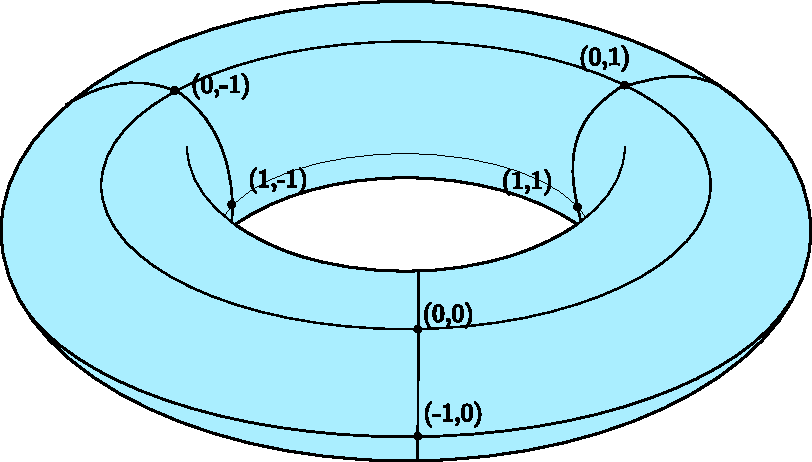
\includegraphics[width=9cm,pagebox=cropbox]{./images/torus_with_3_torsions.pdf}
    \end{center}
    そして$(0,0)$から各頂点への辺を$1$-cycleとして考える.
    こうして考えると,
    level structureを群構造がないcompact Riemann surfaceにも拡張できる.

    \begin{Def}
        $C$ :: curve of genus $g$ over $\C$, $n$ :: positive integerとする.
        $H_1(C^{an}, \Z/n\Z)$を,
        intersection paringをsymplectic formとする
        symplectic vector spaceとみなす.

        $C$のlevel $n$-strcutureとは,
        symplectic isomorphism :: $\alpha: (\Z/n\Z)^{2g} \to H_1(C^{an}, \Z/n\Z)$のことである.
        ここで$(\Z/n\Z)^{2g}$はstanderd symplectic spaceである.

        curves with level structure :: $(C, \alpha), (C', \alpha')$が同型であることを,
        以下のように定める:
        isomorphism :: $\phi: C \to C'$が存在し,
        $\phi$から誘導される写像$\phi^*: H_1(C'^{an}, \Z/n\Z) \to H_1(C'^{an}, \Z/n\Z)$が
        $\phi^* \circ \alpha=\alpha'$を満たす.
    \end{Def}

    以下はより一般の体上のcurveで定義できるlevel structureである.
    O. Bergvall
    ``Cohomology of the moduli space of curves of genus three with level two structure" 
    \footnote{\url{http://www.diva-portal.org/smash/record.jsf?pid=diva2\%3A715000&dswid=5675}}
    Def2.3.1
    からとった.
    \begin{Def}[]
        $k$ :: algebraically closed field,
        $C$ :: smooth, irreducible, and projective curve of genus $g$,
        $n$ :: positive integer with $n \neq \fchar k$とする.
        $n$-torsion points of Jacobi variety of $C$ :: $J(C)[n]$を,
        Weil paringをsymplectic formとする
        symplectic vector spaceとみなす.

        $C$のlevel $n$-structureとは,
        symplectic isomorphism :: $\alpha: (\Z/n\Z)^{2g} \to J(C)[n]$のことである.
        ここで$(\Z/n\Z)^{2g}$はstanderd symplectic spaceである.

        morphism :: $\phi: C \to C'$に対して,
        $\phi^*: J(C') \to J(C)$が誘導される(TODO: HOW?).
        そこで,curves with level structure :: $(C, \alpha), (C', \alpha')$が同型であることを,
        以下のように定める:
        isomorphism :: $\phi: C \to C'$が存在し,
        $\phi^*$が$\phi^* \circ \alpha=\alpha'$を満たす.
    \end{Def}

    \subsubsection{ Weierstrass points }
    こちらを考えても元の問題のmoduli spaceのfinite coverが得られる
    修正としては,
    ordered sets of (higher-order) Weierstrass pointsを考える,
    というものもある.
    Weierstrass pointsの定義は\cite{GAC} pp.41-44にある.
    C. Shor, T. Shaska ``Weierstrass points of superelliptic curves"
    \footnote{\url{https://arxiv.org/pdf/1502.06285.pdf}}
    にも解説がある.

    \subsection{Representation by Algebraic Stacks.}
    moduli functorをschemeで表現できないのなら
    もっと「情報量が多い」もので表現しよう,
    というのが動機である.
    stackはgroupoid(全ての射がisomorphismである圏),
    または2-functor($\Sch^{op}$から圏の圏$\Cat$へのsheaf)として定義される.
    詳細はTom\'as L. G\'omez ``Algebraic stacks"
    \footnote{ \url{ https://arxiv.org/abs/math/9911199 }. }.

\bibliographystyle{jplain}
\bibliography{reference}
\end{document}
